\documentclass{achemso}

\usepackage[T1]{fontenc} 
\usepackage{multirow}
\usepackage{xcolor}
\newcommand{\beginsupplement}{%
        \setcounter{table}{0}
        \renewcommand{\thetable}{S\arabic{table}}%
        \setcounter{figure}{0}
        \renewcommand{\thefigure}{S\arabic{figure}}%
     }

   \usepackage{subcaption}%figure}
\usepackage{verbatim}
\usepackage{minted}
\usepackage{amsmath}
\usepackage{enumerate}

\author{Felippe Mariano Colombari}
\affiliation[Brazilian Nanotechnology National Laboratory]
{Brazilian Nanotechnology National Laboratory, Brazilian Center for
Research in Energy and Materials, Campinas, SP, Brazil}

\author{Kalil Bernardino}
\affiliation[Institute of Chemistry]
{Institute of Chemistry, University of S\~ao Paulo, S\~ao Paulo, SP, Brazil}

\author{Weverson Rodrigues Gomes}
\affiliation[Federal University of S\~ao Carlos]
{Department of Chemistry, Federal University of S\~ao Carlos, S\~ao Carlos, SP, Brazil}

\author{Asdrubal Lozada Blanco}
\affiliation[Federal University of S\~ao Carlos]
{Department of Chemistry, Federal University of S\~ao Carlos, S\~ao Carlos, SP, Brazil}

\author{Andr\'e Farias de Moura}
\email{moura@ufscar.br}
\phone{+55 (16)3351-8090}
\affiliation[Federal University of S\~ao Carlos]
{Department of Chemistry, Federal University of S\~ao Carlos, S\~ao Carlos, SP, Brazil}


\title{\textit{Themis}: a Software to Assess Association Free Energies Via Direct Estimative of Partition Functions}

%%%%%%%%%%%%%%%%%%%%%%%%%%%%%%%%%%%%%%%%%%%%%%%%%%%%%%%%%%%%%%%%%%%%%%%%%%%%%%%%%%%%%%%%%%%%%%%%%%%%%%%%%%%%%%%%%%%%%%%%%%%%%%%%%%%%%%%%%%%%%%%%%%%%%%%%%%%
\begin{document}
\beginsupplement
\footnotesize

\begin{center}
  \textbf{\large{SUPPORTING INFORMATION}}
\end{center}

\clearpage

\begin{center}
  \textbf{\large{\textit{Themis} user guide}}
\end{center}

\noindent

\begin{center}
  \textbf{COMMAND LINE OPTIONS}
\end{center}

  Firstly, to display Themis help, one should use the command below

\begin{center}
  \begin{minipage}{0.7\textwidth}
    \vskip0.25cm
    \begin{minted}[fontsize=\scriptsize,gobble=2,baselinestretch=0.5,escapeinside=!!,frame=lines,framerule=1pt]{bash}

  themis@linux:~$ themis --help

  --------------------------------------------------------------------------

                         Program THEMIS version beta

    STARTED AT: 26/09/2019 - 09:20:23

    COMMAND LINE READ: themis --help

  --------------------------------------------------------------------------

            Usage:  themis [RUNTYPE] [GRIDTYPE] [RADIUS|FILENAME]     

  --------------------------------------------------------------------------

                              [RUNTYPE] options

              --run     Start new calculation.

            --rerun     Read energies from previous run. User must 
                        give an energy.bin file (from Themis) or an 
                        energy.log file (from external programs).

  --------------------------------------------------------------------------

                             [GRIDTYPE] options

            --shell     Translation moves will be performed on a
                        spherical shell grid generated on the run.

             --user     Translation moves will be performed on an
                        user-defined external grid.

  --------------------------------------------------------------------------

                               [RADIUS] value

             (real)     Scaling factor !for! the spherical grid
                        radius (in Angstrom)

                             [FILENAME] value

             (char)     XYZ file containing the user-defined
                        translation grid. It must be aligned
                        with molecule 1

  --------------------------------------------------------------------------

                                Other options

             --help     Display this !help!

          --version     Display the version

  --------------------------------------------------------------------------

  themis@linux:~$

    \end{minted}
  \end{minipage}
\end{center}

  Also, to display Themis license information, one should use the following
  command

\begin{center}
  \begin{minipage}{0.7\textwidth}
    \vskip0.25cm
    \begin{minted}[fontsize=\scriptsize,gobble=2,baselinestretch=0.5,escapeinside=!!,frame=lines,framerule=1pt]{bash}

  themis@linux:~$ themis --license

  --------------------------------------------------------------------------

                         Program THEMIS version beta

    STARTED AT: 26/09/2019 - 10:29:47

    COMMAND LINE READ: themis --license

  --------------------------------------------------------------------------

                Copyright (C) !2019! Felippe Mariano Colombari       

                               License GPLv3+:                     
                         GNU GPL version !3! or later                
                    see <http://gnu.org/license/gpl.html>          

                           This is a free software                 
               you are free to change it and redistributibe it     
             There is NO WARRANTY, to the extent permited by law 

                       Written by Felippe M. Colombari             
                      E-mail: colombarifm@hotmail.com              

  --------------------------------------------------------------------------

  themis@linux:~$ 

    \end{minted}
  \end{minipage}
\end{center}

  To run a new simulation using a spherical translation grid of radius 4.0 \AA,
  one should enter the following command 

\begin{center}
  \begin{minipage}{0.55\textwidth}
    \vskip0.25cm
    \begin{minted}[fontsize=\scriptsize,gobble=2,baselinestretch=0.5,escapeinside=!!,frame=lines,framerule=1pt]{bash}

  themis@linux:~$ themis --run --shell 4.0 > resume.log &
  themis@linux:~$ 

    \end{minted}
  \end{minipage}
\end{center}

  On the other hand, the following command

\begin{center}
  \begin{minipage}{0.55\textwidth}
    \vskip0.25cm
    \begin{minted}[fontsize=\scriptsize,gobble=2,baselinestretch=0.5,escapeinside=!!,frame=lines,framerule=1pt]{bash}

  themis@linux:~$ themis --run --user vdw.xyz > resume.log &
  themis@linux:~$ 

    \end{minted}
  \end{minipage}
\end{center}

  will run a new simulation using a translation grid corresponding to the VdW
  surface of molecule 1 saved on ``vdw.xyz''.

\newpage

\begin{center}
  \textbf{INPUT FILES}
  \vskip0.5cm
\end{center}

%%%%%%%%%%%%%%%%%%%%%%%%%%%%%%%%%%%%%%%%%%%%%%%%%%%%%%%%%%%%%%%%%%%%%%%%%%%%%%%%%%%%%%%%%%%%%%%%%%%%%%%%%%%%%%%%%%%%%%%

\textbf{conf1.xyz} and \textbf{conf2.xyz}: Standard XYZ files containing the
  coordinates of both structures. For the water dimer mentioned in the previous
  sections, a dummy site (X) corresponding to water center of mass was used to
  define an orientation vector along Z-axis, as shown below. \\~

\begin{center}
  \begin{minipage}{0.425\textwidth}
    \begin{minted}[fontsize=\scriptsize,gobble=2,baselinestretch=1.0,escapeinside=!!,frame=lines,framerule=1pt]{bash}

  themis@linux:~$ cat conf1.xyz 

    4 
    *blank line*
    OW      0.00000      0.06682      0.00000
    HW     -0.76677     -0.53032      0.00000
    HW      0.76677     -0.53032      0.00000
    X       0.00000      0.00000      0.00000

  themis@linux:~$ 

    \end{minted}
    \vskip0.5cm
  \end{minipage}%
%
  \hskip1.0cm
%
  \begin{minipage}{0.425\textwidth}
    \begin{minted}[fontsize=\scriptsize,gobble=2,baselinestretch=1.0,escapeinside=!!,frame=lines,framerule=1pt]{bash}

  themis@linux:~$ cat conf2.xyz 

    4 
    *blank line*
    OW      0.00000      0.06682      0.00000
    HW     -0.76677     -0.53032      0.00000
    HW      0.76677     -0.53032      0.00000
    X       0.00000      0.00000      0.00000

  themis@linux:~$

    \end{minted}
    \vskip0.5cm
  \end{minipage}%
\end{center}

%%%%%%%%%%%%%%%%%%%%%%%%%%%%%%%%%%%%%%%%%%%%%%%%%%%%%%%%%%%%%%%%%%%%%%%%%%%%%%%%%%%%%%%%%%%%%%%%%%%%%%%%%%%%%%%%%%%%%%%

\textbf{parameters1} and \textbf{parameters2} are plain text files containing
potential parameters used for energy calculations. Those files are read differently 
according to the potential used. For \texttt{potential : lj-coul} (eq.~\ref{eqn:ljc}), 
TIP3P water parameters are given as follows:

\begin{equation}
  \label{eqn:ljc}
  U_{\textrm{ljc}} = U_{\textrm{lj}} + U_{\textrm{coul}} = 
  \sum\limits_{i} \sum\limits_{j<i}4\epsilon_{ij}\bigg(\bigg(\frac{\sigma_{ij}}{r_{ij}}\bigg)^{\!\!12}
  -\bigg(\frac{\sigma_{ij}}{r_{ij}}\bigg)^{\!\!6}\bigg)
	+\frac{1}{4\pi\epsilon_{0}}\sum\limits_{i} \sum\limits_{j<i}\frac{q_{i}q_{j}}{r_{ij}}
\end{equation}

where $\epsilon_{ij} = ( \epsilon_{i} \cdot \epsilon_{j})^\frac{1}{2}$ and
$\sigma_{ij} = ( \sigma_{i} \cdot \sigma_{j})^\frac{1}{2}$

\begin{center}
  \begin{minipage}{0.425\textwidth}
    \vskip0.25cm
    \begin{minted}[fontsize=\scriptsize,gobble=2,baselinestretch=1.0,escapeinside=!!,frame=lines,framerule=1pt]{bash}

  themis@linux:~$ cat parameters1

   q          sig (A)     eps (kJ/mol)
OW -0.834     3.15061     0.636386
HW +0.417     0.00000     0.000000	 
HW +0.417     0.00000     0.000000	 
X   0.000     0.00000     0.000000

  themis@linux:~$

    \end{minted}
  \end{minipage}%
%
  \hskip0.5cm
%
  \begin{minipage}{0.425\textwidth}
    \vskip0.25cm
    \begin{minted}[fontsize=\scriptsize,gobble=2,baselinestretch=1.0,escapeinside=!!,frame=lines,framerule=1pt]{bash}

  themis@linux:~$ cat parameters2

   q          sig (A)     eps (kJ/mol)
OW -0.834     3.15061     0.636386
HW +0.417     0.00000     0.000000	 
HW +0.417     0.00000     0.000000	 
X   0.000     0.00000     0.000000

  themis@linux:~$

    \end{minted}
  \end{minipage}%
\end{center}

  For \texttt{potential : bh-coul} (eq.~\ref{eqn:bhc}), MATSUI parameters 
for a TiO$_{2}$ unit must be provided as follows:

\begin{equation}
  \label{eqn:bhc}
  U_{\textrm{bhc}} = U_{\textrm{bh}} + U_{\textrm{coul}} = 
  \sum\limits_{i}
  \sum\limits_{j<i}\bigg\{\bigg(\frac{-C_{i}C_{j}}{r_{ij}^{6}}\bigg)
  + f(B_{i}+B_{j})
\exp\bigg[\bigg(\frac{A_{i}+A_{j}-r_{ij}}{B_{i}+B_{j}}\bigg)\bigg]\bigg\}
	+\frac{1}{4\pi\epsilon_{0}}\sum\limits_{i} \sum\limits_{j<i}\frac{q_{i}q_{j}}{r_{ij}}
\end{equation}

  where the quantity $f$ corresponds to a standard force of 4.184 kJ/mol/\AA. 

\begin{center}
  \begin{minipage}{0.425\textwidth}
    \vskip0.25cm
    \begin{minted}[fontsize=\scriptsize,gobble=2,baselinestretch=1.0,escapeinside=!!,frame=lines,framerule=1pt]{bash}

  themis@linux:~$ cat parameters1

    q          A(A)      B (A)     C(A^3 kJ/mol)
Ti   2.1960    1.18230   0.07700   22.5000
O   -1.0980    1.63390   0.11700   54.0000
O   -1.0980    1.63390   0.11700   54.0000
X    0.0000    0.00000   0.00000   0.00000

  themis@linux:~$

    \end{minted}
  \end{minipage}%
%
  \hskip0.75cm
%
  \begin{minipage}{0.425\textwidth}
    \vskip0.25cm
    \begin{minted}[fontsize=\scriptsize,gobble=2,baselinestretch=1.0,escapeinside=!!,frame=lines,framerule=1pt]{bash}

  themis@linux:~$ cat parameters2

    q          A(A)      B (A)     C(A^3 kJ/mol)
Ti  2.1960    1.18230   0.07700   22.5000
O  -1.0980    1.63390   0.11700   54.0000
O  -1.0980    1.63390   0.11700   54.0000
X   0.0000    0.00000   0.00000   0.00000

  themis@linux:~$

    \end{minted}
  \end{minipage}%
\end{center}

  NOTE: It is important to highlight that atoms described in both \texttt{parameters1}
and \texttt{parameters2} files MUST BE IN THE SAME ORDER as they appear in both 
\texttt{conf1.xyz} and \texttt{conf2.xyz} files. Parameters file MUST contain a 
header followed by one line for each atom descrived in structure files.

%%%%%%%%%%%%%%%%%%%%%%%%%%%%%%%%%%%%%%%%%%%%%%%%%%%%%%%%%%%%%%%%%%%%%%%%%%%%%%%%%%%%%%%%%%%%%%%%%%%%%%%%%%%%%%%%%%%%%%%

\newpage
\textbf{INPUT file}: plain text file containing detailed intructions prior to
calculation. 

\begin{center}
  \begin{minipage}{0.95\textwidth}
    \vskip0.25cm
    \begin{minted}[fontsize=\scriptsize,gobble=2,baselinestretch=1.0,escapeinside=!!,frame=lines,framerule=1pt]{bash}

  themis@linux:~$ cat INPUT 

    reorientation_factor : 2                    !#! integer
    translation_factor : 2                      !#! integer
    gyration_factor :  36                       !#! integer
    gyration_range : 360.0                      !#! real 
    temperature : 300.0                         !#! real
    potential : lj-coul                         !#! character. valid strings are: none, lj-coul our bh-coul
    ref_mol1 : 1                                !#! integer
    rot_ref_mol1 : 4                            !#! integer
    ref_mol2 : 1                                !#! integer
    rot_ref_mol2 : 2                            !#! integer
    shortest_distance : 0.8                     !#! real
    write_xtc : no                              !#! character. valid strings are: no, F, yes or T
    lowest_structures : 20                      !#! integer
    write_frames : none                         !#! character. valid strings are: none, MOP or XYZ
    mopac_job :                                 !#! character

  themis@linux:~$

    \end{minted}
  \end{minipage}%
\end{center}

\texttt{reorientation\_factor}: Parameter ($p$) used to generate the spherical 
  grid used for reorientation moves. The number of points ($n$) obtained along 
  the sphere surface by dodecahedron tessellation is given by
  $$ n = 12 + 10 \times 3 \times ( p - 1 ) + 10 \times ( p - 2 ) \times ( p - 1 ) $$
  If one uses $p = 0$, the reorientation move will correspond to align molecule 2 along 
  Z-axis (1 reorientational move). 

\begin{figure}[!h]
  \begin{subfigure}[t]{0.18\textwidth}
    \center
    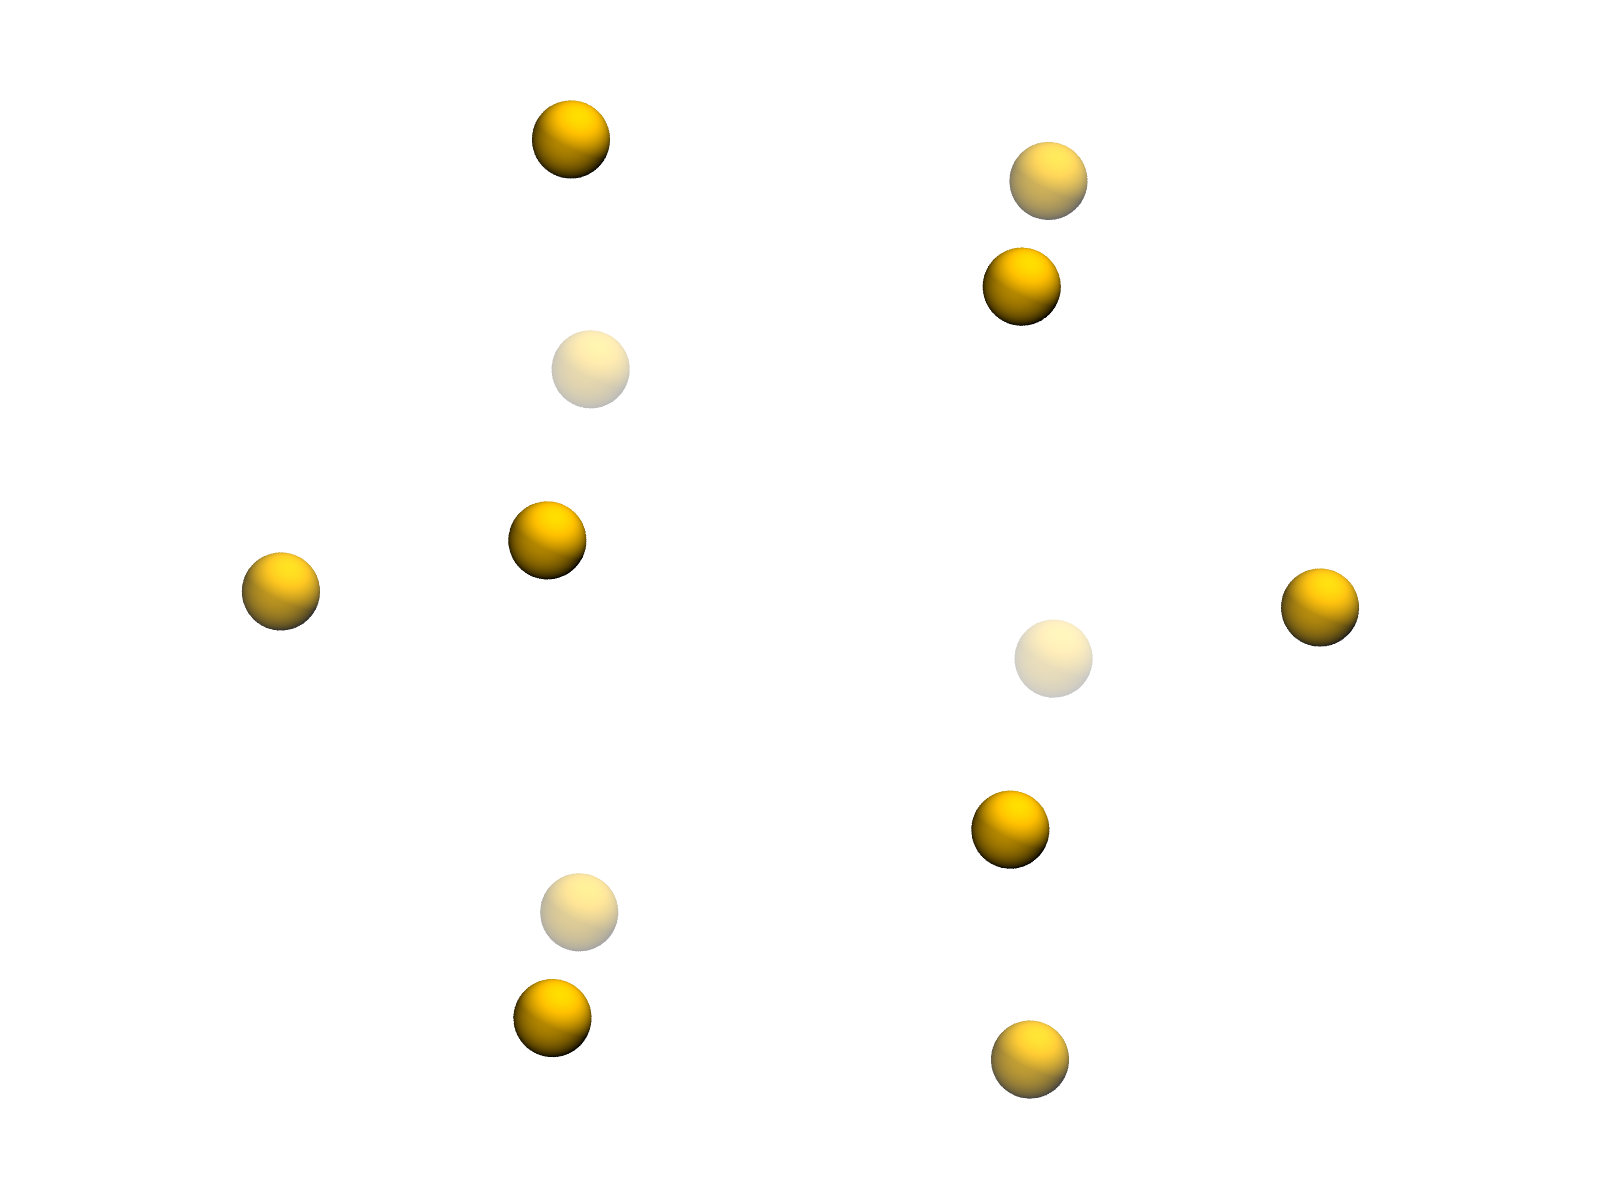
\includegraphics[width=\textwidth]{../HIGH_RES_IMAGES/grid_012.png}
    \footnotesize
    $p = 1$ \\
    $n = 12$
  \end{subfigure}
  \begin{subfigure}[t]{0.18\textwidth}
    \center
    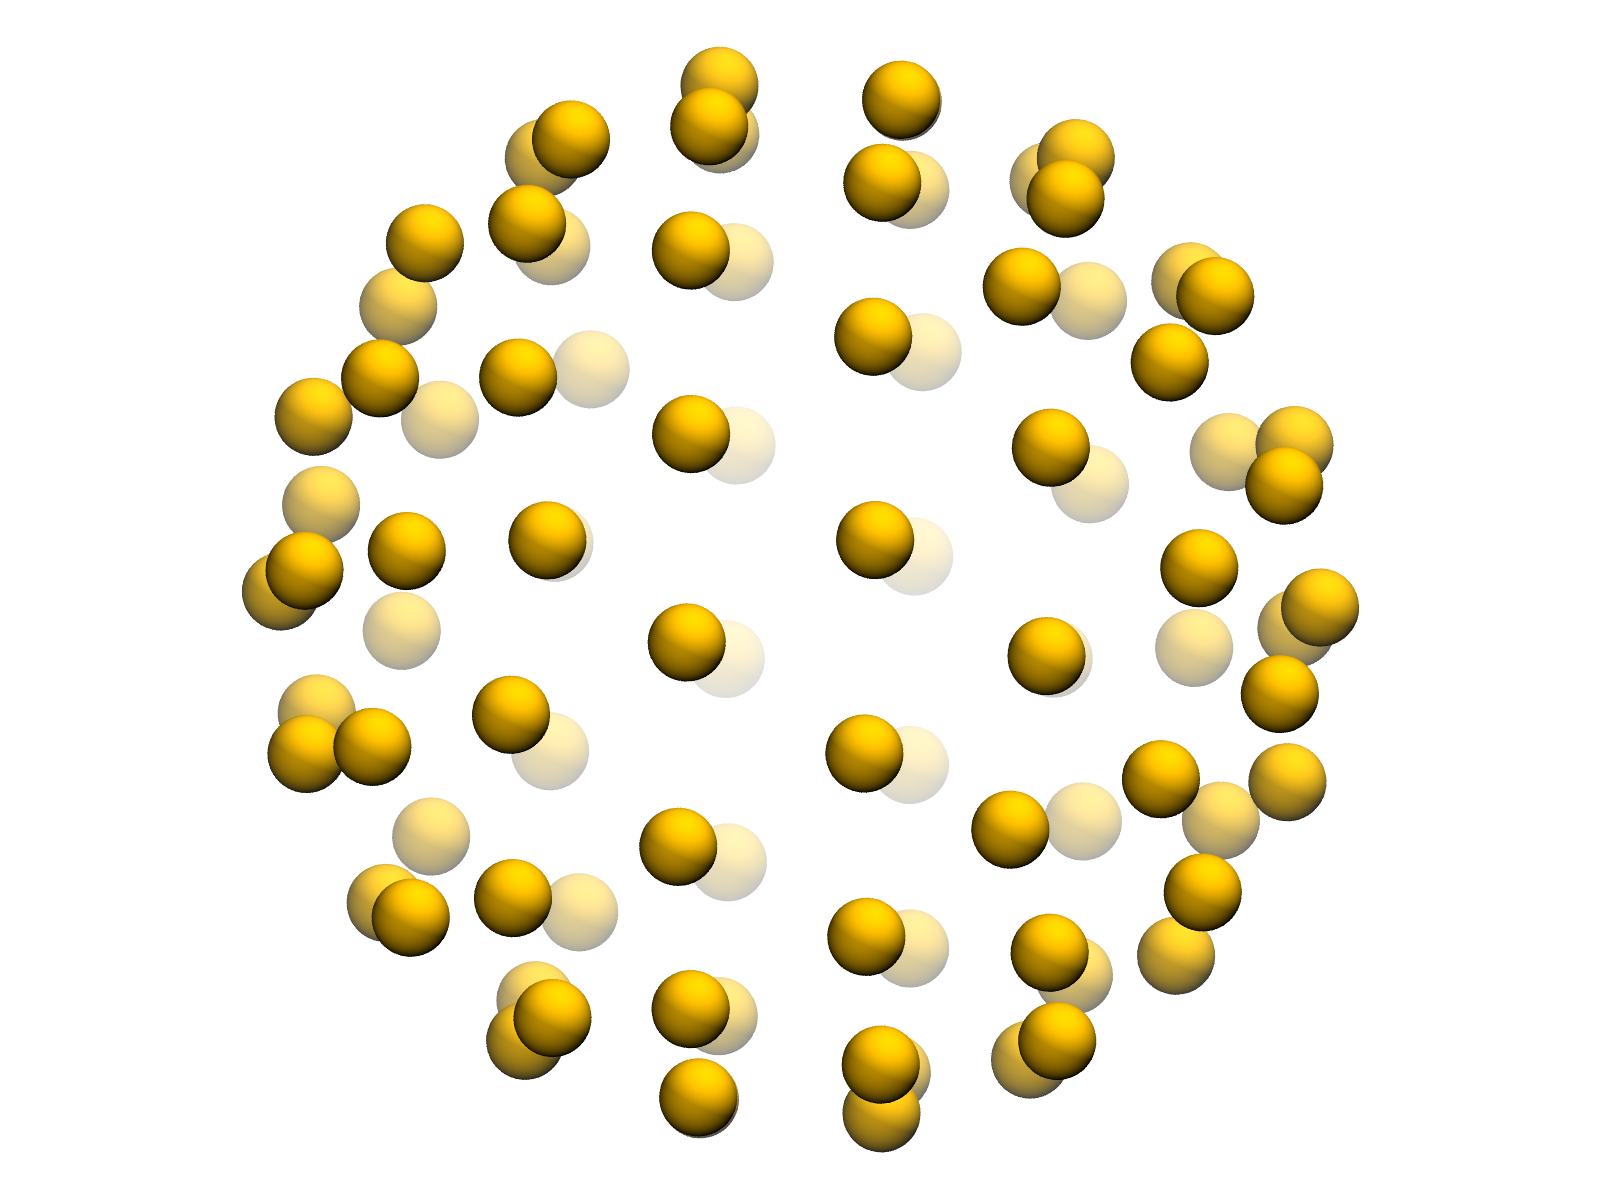
\includegraphics[width=\textwidth]{../HIGH_RES_IMAGES/grid_092.png} 
    \footnotesize
    $p = 3$ \\
    $n = 92$
  \end{subfigure}
  \begin{subfigure}[t]{0.18\textwidth}
    \center
    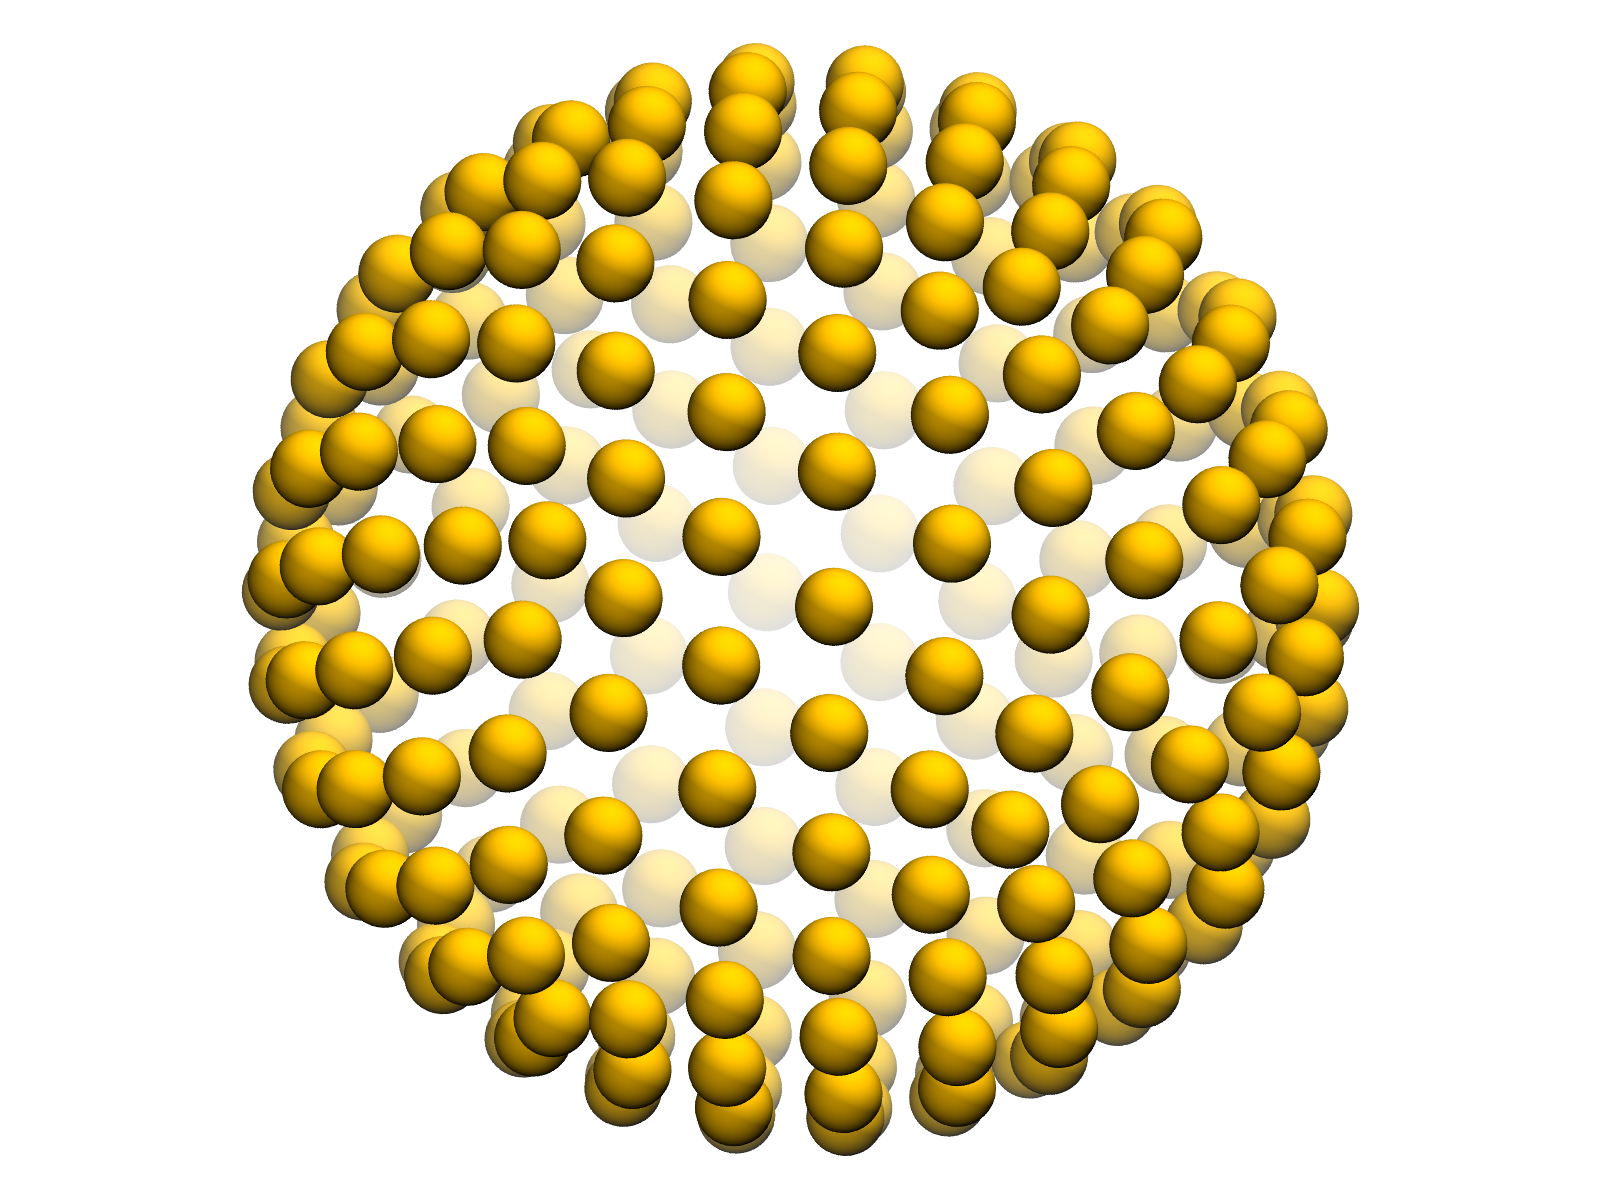
\includegraphics[width=\textwidth]{../HIGH_RES_IMAGES/grid_252.png} 
    \footnotesize
    $p = 5$ \\
    $n = 252$
  \end{subfigure}
  \begin{subfigure}[t]{0.18\textwidth}
    \center
    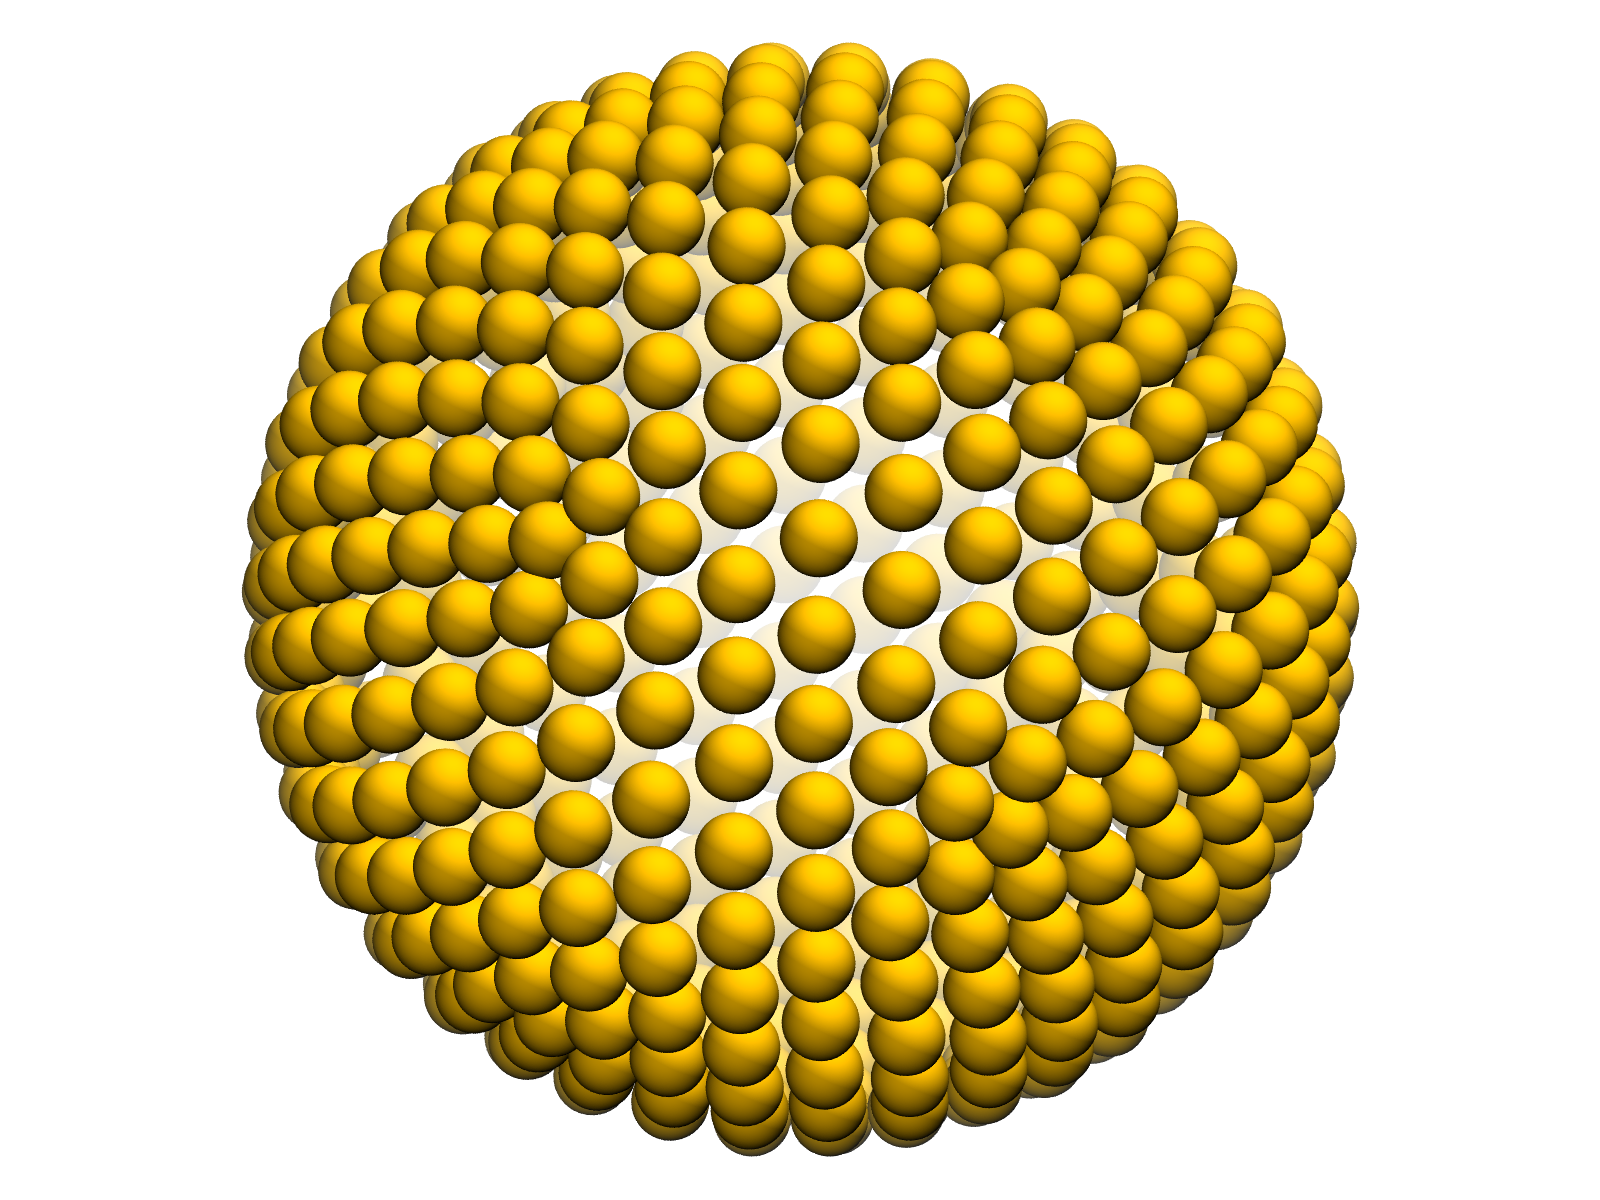
\includegraphics[width=\textwidth]{../HIGH_RES_IMAGES/grid_492.png} 
    \footnotesize
    $p = 7$ \\
    $n = 492$
  \end{subfigure}
  \begin{subfigure}[t]{0.18\textwidth}
    \center
    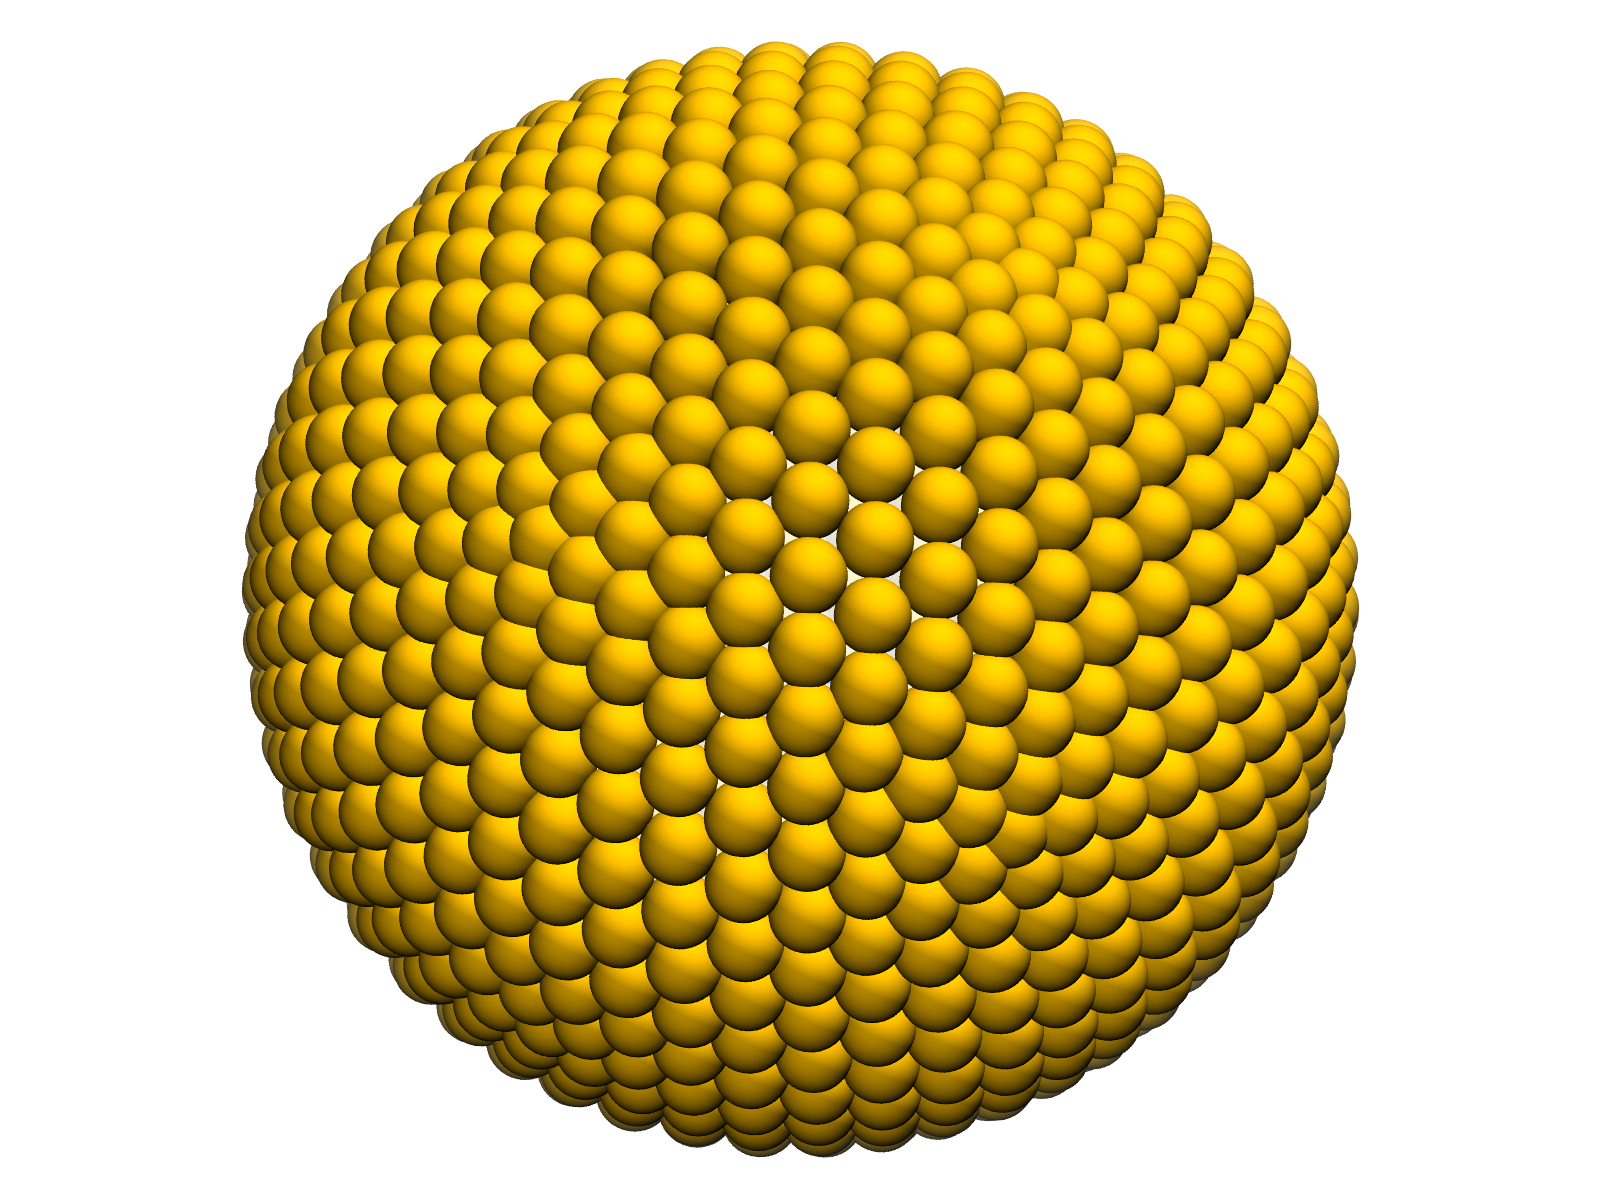
\includegraphics[width=\textwidth]{../HIGH_RES_IMAGES/grid_812.png} 
    \footnotesize
    $p = 9$ \\
    $n = 812$
  \end{subfigure}
\end{figure}

\texttt{translation\_factor}: Same as \texttt{reorientation\_grid} if a spherical
  translation shell is used.

\texttt{gyration\_factor}:  Corresponds to the number of gyration points around
  the rotation axis. 
  
\texttt{gyration\_range}: Corresponds to the maximum rotation angle (in degrees). 

\texttt{temperature}: Absolute temperature (K). 

\texttt{potential}: Potential energy function selection. Options are ``none'', 
  ``lj-coul'', ``bh-coul''. 

\texttt{write\_frames}: Selects the format in which all valid frames will be
  written: ``XYZ'', ``MOP'' and ``none''. If ``MOP'' is selected, the optional
  character variable containing the first line of MOPAC input is read. 

\texttt{ref\_mol1}: Site of molecule 1 used for centering, according to
  \texttt{conf1.xyz} file. 

\texttt{rot\_ref\_mol1}: Site of molecule 1 that will build its rotation
  vector, according to \texttt{conf1.xyz} file. 

\texttt{ref\_mol2}: Site of molecule 2 used for centering, according to
  \texttt{conf2.xyz} file. 

\texttt{rot\_ref\_mol2}: Site of molecule 2 that will build its rotation
  vector, according to \texttt{conf2.xyz} file. 

\texttt{shortest\_distance}: Corresponds to the lowest intermolecular distance
  to consider the configuration as a valid one. Below such value (in Angstrom), 
  molecular contacts are considered strongly repulsive and an interaction energy 
  value of $10^{10}$ kJ/mol is attributed  to such configuration. This is useful 
  to avoid spending time calculating energies for unphisical configurations since 
  the energy loop is skipped.

\texttt{write\_xtc}: Flag to enable the writting of all configurations to
  a XTC file. WARNING: very large files can be generated ;) 
  
\texttt{lowest\_structures}: selects the number of lowest energy/highest
  probability structures to write after the run. 
  
\texttt{mopac\_job}: string containing the header for mopac calculations.
  enabled when ``write\_frames : MOP'' is selected.

%%%%%%%%%%%%%%%%%%%%%%%%%%%%%%%%%%%%%%%%%%%%%%%%%%%%%%%%%%%%%%%%%%%%%%%%%%%%%%%%%%%%%%%%%%%%%%%%%%%%%%%%%%%%%%%%%%%%%%%

\newpage

\begin{center}
  \textbf{OUTPUT FILES}
\end{center}

\textbf{energy.bin}

  Binary file containing interaction energy values for all microstates. Since
  all entries are written in the right loop sequence, they can be read using the
  \texttt{rerun} feature. \\~

\textbf{energy-sort.log}
  
  Contains interaction energy values and probabilities for the N most probable
  structures. By running Themis with the input files presented below, and
  considering a spherical grid with radius = 2.8 \AA, one obtains \\~

\begin{center}
  \begin{minipage}{0.65\textwidth}
    \vskip0.25cm
    \begin{minted}[fontsize=\scriptsize,gobble=2,baselinestretch=1.0,escapeinside=!!,frame=lines,framerule=1pt]{bash}

  themis@linux:~$ cat energy-sort.log

  inter_energy(g,r,t)   g       r       t        prob.     sum prob.
    -2.83500E+001       1      10       3     6.704E-004  6.704E-004
    -2.83500E+001       1       4       9     6.704E-004  1.341E-003
    -2.83453E+001       2       4       9     6.692E-004  2.010E-003
    -2.83453E+001       2      10       3     6.692E-004  2.679E-003
    -2.83453E+001     120       4       9     6.692E-004  3.348E-003
    -2.83453E+001     120      10       3     6.692E-004  4.017E-003
    -2.83312E+001       3      10       3     6.654E-004  4.683E-003
    -2.83312E+001     119      10       3     6.654E-004  5.348E-003
    -2.83312E+001       3       4       9     6.654E-004  6.014E-003
    -2.83312E+001     119       4       9     6.654E-004  6.679E-003
    -2.83078E+001     118      10       3     6.592E-004  7.338E-003
    -2.83078E+001     118       4       9     6.592E-004  7.997E-003
    -2.83078E+001       4      10       3     6.592E-004  8.657E-003
    -2.83078E+001       4       4       9     6.592E-004  9.316E-003
    -2.82751E+001     117       4       9     6.506E-004  9.966E-003
    -2.82751E+001     117      10       3     6.506E-004  1.062E-002
    -2.82751E+001       5      10       3     6.506E-004  1.127E-002
    -2.82751E+001       5       4       9     6.506E-004  1.192E-002
    -2.82333E+001     116      10       3     6.398E-004  1.256E-002
    -2.82333E+001       6      10       3     6.398E-004  1.320E-002

  themis@linux:~$ 

    \end{minted}
  \end{minipage}%
\end{center}

\textbf{output.log}

  Contains thermodynamic data for all translation grid points, and also for the
  overall ensemble. Written in an extended XYZ format containing extra field values 
  for each grid point (probability, free energy, energy and entropic penalty). \\~


\begin{center}
  \begin{minipage}{0.95\textwidth}
    \vskip0.25cm
    \begin{minted}[fontsize=\scriptsize,gobble=2,baselinestretch=1.0,escapeinside=!!,frame=lines,framerule=1pt]{bash}

  themis@linux:~$ cat output.log

        42
       X (A)     Y (A)     Z (A)  point           PROB      A (kJ/mol)    -TS (kJ/mol)      E (kJ/mol)
X    2.38182   1.47205   0.00000      1   2.98845E-003   -1.08134E+001    6.75915E+000   -1.75725E+001
X    2.38182  -1.47205   0.00000      2   2.98845E-003   -1.08134E+001    6.75915E+000   -1.75725E+001
X    1.47205   0.00000   2.38182      3   5.85172E-002   -1.82330E+001    6.84167E+000   -2.50746E+001
X    1.47205   0.00000  -2.38182      4   1.34004E-003   -8.81280E+000    4.19575E+000   -1.30086E+001
X    0.00000   2.38182   1.47205      5   1.00969E-002   -1.38502E+001    6.78551E+000   -2.06357E+001
X    0.00000   2.38182  -1.47205      6   1.74725E-001   -2.09615E+001    4.32032E+000   -2.52818E+001
X    0.00000  -2.38182   1.47205      7   1.00969E-002   -1.38502E+001    6.78551E+000   -2.06357E+001
X    0.00000  -2.38182  -1.47205      8   1.74725E-001   -2.09615E+001    4.32032E+000   -2.52818E+001
...
X   -2.26525   0.86525  -1.40000     40   9.83462E-004   -8.04111E+000    5.57165E+000   -1.36128E+001
X   -2.26525  -0.86525  -1.40000     41   9.83462E-004   -8.04111E+000    5.57165E+000   -1.36128E+001
X   -2.80000   0.00000   0.00000     42   2.97201E-003   -1.07996E+001    6.97190E+000   -1.77715E+001
-------------------------------------------------------------------------------------------------------
TOTAL OVER TRANSLATIONAL GRID             1.00000E+000   -1.59900E+001    7.67496E+000   -2.36649E+001

  themis@linux:~$ 

    \end{minted}
  \end{minipage}%
\end{center}

\textbf{output-sort.log}

  Same as \texttt{output.log} but ordered from most probable point to the least 
  probable point. \\~ 

\begin{center}
  \begin{minipage}{0.95\textwidth}
    \begin{minted}[fontsize=\scriptsize,gobble=2,baselinestretch=1.0,escapeinside=!!,frame=lines,framerule=1pt]{bash}

  themis@linux:~$ cat output-sort.log

       42
       X (A)     Y (A)     Z (A)  point           PROB      A (kJ/mol)    -TS (kJ/mol)      E (kJ/mol)
X    0.00000  -2.38182  -1.47205      8   1.74725E-001   -2.09615E+001    4.32032E+000   -2.52818E+001
X    0.00000   2.38182  -1.47205      6   1.74725E-001   -2.09615E+001    4.32032E+000   -2.52818E+001
X    0.00000   0.00000   2.80000     24   8.68520E-002   -1.92179E+001    6.43659E+000   -2.56545E+001
X    1.47205   0.00000   2.38182      3   5.85172E-002   -1.82330E+001    6.84167E+000   -2.50746E+001
X   -1.47205   0.00000   2.38182      9   5.85172E-002   -1.82330E+001    6.84167E+000   -2.50746E+001
X    0.86525   1.40000   2.26525     22   4.04675E-002   -1.73130E+001    7.12969E+000   -2.44427E+001
X   -0.86525   1.40000   2.26525     29   4.04675E-002   -1.73130E+001    7.12969E+000   -2.44427E+001
X    0.86525  -1.40000   2.26525     23   4.04675E-002   -1.73130E+001    7.12969E+000   -2.44427E+001
...
X   -2.26525   0.86525  -1.40000     40   9.83462E-004   -8.04111E+000    5.57165E+000   -1.36128E+001
X    2.26525  -0.86525  -1.40000     19   9.83462E-004   -8.04111E+000    5.57165E+000   -1.36128E+001
X   -2.26525  -0.86525  -1.40000     41   9.83462E-004   -8.04111E+000    5.57165E+000   -1.36128E+001
-------------------------------------------------------------------------------------------------------
TOTAL OVER TRANSLATIONAL GRID             1.00000E+000   -1.59900E+001    7.67496E+000   -2.36649E+001

  themis@linux:~$ 

    \end{minted}
    \vskip0.25cm
  \end{minipage}%
\end{center}

\textbf{surf\_free-energy.vmd, surf\_energy.vmd, surf\_entropic-penalty.vmd} 

  Contains a VMD script for reading the thermodynamic data along the translation
  grid from file \texttt{output.log}. \\~

\textbf{lowest\_0001.xyz}
  
  XYZ coordinates for the most probable structure from the whole ensemble. The
  number of lowest structure files is defined by the user in the \texttt{INPUT}
  file. \\~

\begin{center}
  \begin{minipage}{0.4\textwidth}
    \begin{minted}[fontsize=\scriptsize,gobble=2,baselinestretch=1.0,escapeinside=!!,frame=lines,framerule=1pt]{bash}

  themis@linux:~$ cat lowest_0001.xyz

           8
Energy =  -2.8350000E+01
 O       0.0000     0.0000     0.0000
 H      -0.0000    -0.7668    -0.5971
 H      -0.0000     0.7668    -0.5971
 X      -0.0000    -0.0000    -0.0668
 O       1.4720     0.0000     2.3818
 H       0.9611     0.0000     1.5551
 H       0.7957     0.0000     3.0797
 X       1.4056     0.0000     2.3746

  themis@linux:~$ 

    \end{minted}
    \vskip0.25cm
  \end{minipage}%
\end{center}


\textbf{grid\_log.log}

  File containing informations of each translation grid point: point number,
number of rejected structures, spent time. \\~

\begin{center}
  \begin{minipage}{0.4\textwidth}
    \begin{minted}[fontsize=\scriptsize,gobble=2,baselinestretch=1.0,escapeinside=!!,frame=lines,framerule=1pt]{bash}

  themis@linux:~$ cat grid_log.log

t point   rejected structures   time (s)
      1         0 of    5040      0.020
      2         0 of    5040      0.012
      3         0 of    5040      0.012
      4         0 of    5040      0.013
...
     38         0 of    5040      0.024
     39         0 of    5040      0.013
     40         0 of    5040      0.013
     41         0 of    5040      0.012
     42         0 of    5040      0.014

  themis@linux:~$ 

    \end{minted}
    \vskip0.25cm
  \end{minipage}%
\end{center}

\textbf{full\_ensemble.xtc}

  XTC trajectory file containing the whole ensemble. Written if INPUT option
  \texttt{write\_xtc} is enabled. \\~

\textbf{point\_0001\_0001\_0001.xyz}

  XYZ file containing the structure of the microstate t = 1, r = 1, g = 1. Files
are numbered according to the loop position. Written if INPUT option
\texttt{write\_frames = XYZ} is set. Microstates with intermolecular distances 
below the one defined by \texttt{shortest\_distance} are skipped. WARNING: this 
option will create a very large number of files in the directory. ;) \\~ 

\begin{center}
  \begin{minipage}{0.4\textwidth}
    \begin{minted}[fontsize=\scriptsize,gobble=2,baselinestretch=1.0,escapeinside=!!,frame=lines,framerule=1pt]{bash}

  themis@linux:~$ point_0001_0001_0001.xyz

           8
Energy =   0.0000000E+00
 O       0.0000     0.0000     0.0000
 H      -0.0000    -0.7668    -0.5971
 H      -0.0000     0.7668    -0.5971
 X      -0.0000    -0.0000    -0.0668
 O       2.3818     1.4720     0.0000
 H       3.2085     1.9830    -0.0000
 H       2.1793     1.3469     0.9423
 X       2.4167     1.4936     0.0527


  themis@linux:~$ 

    \end{minted}
    \vskip0.25cm
  \end{minipage}%
\end{center}

\textbf{point\_0001\_0001\_0001.mop}
  
  Same as before, but in MOPAC format, containing the header defined by 
\texttt{mopac\_job}. Written if INPUT options \texttt{write\_frames = MOP} is 
set. Microstates with intermolecular distances below the one defined by 
\texttt{shortest\_distance} are skipped. WARNING: this option will create a 
very large number of files in the directory. ;) \\~ 

\begin{center}
  \begin{minipage}{0.4\textwidth}
    \begin{minted}[fontsize=\scriptsize,gobble=2,baselinestretch=1.0,escapeinside=!!,frame=lines,framerule=1pt]{bash}

  themis@linux:~$ point_0001_0001_0001.mop

 PM7 1SCF CHARGE=0 THREADS=1 OUTPUT
*blank line*
*blank line*
 O       0.0000  0   0.0000  0   0.0000  0
 H      -0.0000  1  -0.7668  1  -0.5971  1
 H      -0.0000  1   0.7668  1  -0.5971  1
 X      -0.0000  0  -0.0000  0  -0.0668  0
 O       2.3818  0   1.4720  0   0.0000  0
 H       3.2085  0   1.9830  0  -0.0000  0 
 H       2.1793  1   1.3469  1   0.9423  1
 X       2.4167  1   1.4936  1   0.0527  1

  themis@linux:~$ 

    \end{minted}
    \vskip0.25cm
  \end{minipage}%
\end{center}

\clearpage

\begin{center}
  \textbf{\large{Umbrella Sampling calculations for the water dimer}}
\end{center}

  The sampling along the OW-OW separation coordinate ($\xi$) was carried by running multiple
  independent simulations with a biased umbrella potential that restrains the
  water-water intermolecular distance. For each run, a short energy minimization
  was carried in order to remove repulsive contacts (especially for short
  intermolecular distances). The sampling was carried out in vacuum using a stochastic 
  dynamics integrator (T = 300 K). Lennard-Jones and electrostatic interactions were 
  computed in direct space without a cutoff. Bonds were constrained using LINCS allowing 
  a time step of 2 fs. $\xi_{i}$ was sampled from {2 \AA} to {15 \AA} in {0.5
  \AA} intervals. An umbrella force constant of $10^{4}$ kJ/mol/nm$^{2}$
  was set for {3 \AA} $\leq \xi_{i} \leq$ {15 \AA}, and 2 $\times 10^{4}$ kJ/mol/nm$^{2}$
  for {2 \AA} $\leq \xi_{i} <$ {3 \AA}.

  Entropic and energetic contributions to the potential of mean force can be obtained by 
  finite differences, considering simulations at different
  temperatures (here, 275 K and 325K).

  $$ \Delta S(\xi) = - \Bigg( \dfrac{\partial \Delta A (\xi , T)}{\partial T} \Bigg) $$

  $$ \Delta S(\xi) = - \dfrac{ [\Delta A (\xi , T+\Delta T) - \Delta A (\xi , T-\Delta T]}{2 \Delta T} $$


\clearpage

{
\color{red}{

\begin{center}
  \textbf{\large{Workflow for MOPAC calculations of biphenyl dimers}}
\end{center}

  Calculations using Themis + MOPAC were performed in multiple steps. For each
  intermolecular distance

  \begin{enumerate}[i)]

  \item Write MOPAC input files for all configurations using the following INPUT
    options: \\

\begin{center}
  \begin{minipage}{0.65\textwidth}
    \vskip0.25cm
    \begin{minted}[fontsize=\scriptsize,gobble=2,baselinestretch=1.0,escapeinside=!!,frame=lines,framerule=1pt]{bash}

  themis@linux:~$ cat INPUT 

    reorientation_factor : 4                
    translation_factor : 3                 
    gyration_factor :  36                 
    gyration_range : 360.0               
    temperature : 300.0                 
    potential : none                   
    ref_mol1 : 23                     
    rot_ref_mol1 : 1                 
    ref_mol2 : 23                   
    rot_ref_mol2 : 1               
    shortest_distance : 1.2       
    write_xtc : no               
    lowest_structures : 10      
    write_frames : none        
    mopac_job : MOP PM7 1scf output threads=1 shift=1.0 itry=150

  themis@linux:~$

    \end{minted}
  \end{minipage}%
\end{center}

  \item Run the single-point calculation for every \texttt{.mop} file. This can
    be done more efficiently using the GNU Parallel tool. \\

  \item Once finished, a python script was used to extract the final heat of
    formation of every output file and generate a \texttt{energy.log} file containing all
    interaction energies. \\

  \item Themis \texttt{--rerun} option was used to read all required files,
    calculate all thermodynamic properties and search for the most stable
    structures.\\

\end{enumerate}

  For excited state calculations, we used the following MOPAC header:

\begin{center}
  \begin{minipage}{0.95\textwidth}
    \vskip0.25cm
    \begin{minted}[fontsize=\scriptsize,gobble=2,baselinestretch=1.0,escapeinside=!!,frame=lines,framerule=1pt]{bash}

    mopac_job : MOP PM7 1scf output threads=1 shift=1.0 itry=150 CIS C.I.=4 MECI ROOT=2 SINGLET geo-ok 

    \end{minted}
  \end{minipage}%
\end{center}
}

\end{document}


